\documentclass[11pt]{article}
\usepackage[a4paper,margin=25mm]{geometry}
\usepackage[T1]{fontenc}
\usepackage[utf8]{inputenc}
\usepackage{lmodern,microtype}
\usepackage{amsmath,amssymb,amsfonts,amsthm,mathtools,bm}
\usepackage{booktabs,longtable,array,tabularx,multirow}
\usepackage{graphicx,xcolor,enumitem}
\usepackage{tikz}
\usetikzlibrary{arrows.meta,positioning,calc,fit,backgrounds,shapes.geometric}
\usepackage{algorithm}
\usepackage[noend]{algpseudocode}
\usepackage{hyperref}
\usepackage[nameinlink,noabbrev]{cleveref}
\usepackage[numbers,sort&compress]{natbib}
\usepackage{authblk}
\usepackage{fancyhdr}
\usepackage{caption}
\usepackage{subcaption}
\usepackage{listings}
\usepackage{url}
\hypersetup{colorlinks=true,linkcolor=blue!55!black,citecolor=green!40!black,urlcolor=blue!60!black,pdftitle={Symplectic Transport, Dissipative Learning, and Fisher--Rao Control for MMALS}}
\pagestyle{fancy}\setlength{\headheight}{14pt}\fancyhf{}\lhead{MMALS Symplectic Dynamics}\rhead{Harbonnier}\cfoot{\thepage}
\newtheorem{theorem}{Theorem}
\newtheorem{proposition}{Proposition}
\newtheorem{lemma}{Lemma}
\newtheorem{corollary}{Corollary}
\theoremstyle{definition}\newtheorem{definition}{Definition}\newtheorem{assumption}{Assumption}
\theoremstyle{remark}\newtheorem{remark}{Remark}
\newcommand{\R}{\mathbb{R}}\newcommand{\C}{\mathbb{C}}\newcommand{\E}{\mathbb{E}}
\newcommand{\Sp}{\mathrm{Sp}}\newcommand{\Orth}{\mathrm{O}}\newcommand{\U}{\mathrm{U}}
\newcommand{\FR}{\mathrm{FR}}\newcommand{\KL}{\mathrm{KL}}\newcommand{\diag}{\mathrm{diag}}
\newcommand{\norm}[1]{\left\lVert #1\right\rVert}\newcommand{\ip}[2]{\left\langle #1,#2\right\rangle}
\newcommand{\dd}{\mathrm{d}}\newcommand{\T}{^{\mathsf T}}
\definecolor{mmalsgreen}{RGB}{46,102,76}\definecolor{mmalsgold}{RGB}{181,140,55}\definecolor{mmalsblue}{RGB}{46,79,123}
\title{\textbf{Symplectic Transport, Dissipative Learning, and Fisher--Rao Control for MMALS}\\\large A Geometric Foundation for Adaptive Host Networks Beyond the Unitary Subspace}
\author[1]{Guillaume Harbonnier}
\affil[1]{Independent MMALS Research Program\\\texttt{https://github.com/gharbonnier78}}
\date{Version 0.1.0 -- June 2026}
\begin{document}
\maketitle

\begin{abstract}
Volovich's proposal of symplectic computation starts from a valid but incomplete observation: finite-dimensional Schrödinger evolution admits an exact real Hamiltonian representation, and the unitary group embeds into the orthogonal-symplectic subgroup. This geometric inclusion does not by itself establish greater computational power, because a meaningful comparison also requires a measurement model, a finite-precision resource model, and explicit accounting of gain, dynamic range, noise, and control energy. We develop a rigorous synthesis between that observation and the current MMALS research program. The resulting framework treats symplectic geometry as a reversible transport layer, port-Hamiltonian dissipation as a stabilization and consolidation layer, Fisher--Rao geometry as the statistical learning layer, and goal-conditioned control as the mechanism that shapes resource allocation and action. We correct the tensor-product dimension issue in the original symbit discussion, distinguish rebits from full qubits, formulate a hybrid host-network state space, derive energy-balance and passivity statements, specify an auditable computational trace, and propose a staged experimental program linked to continual learning, inferred-context routing, geometry-aware memory, goal switching, and conformal action gating. The article makes no unconditional claim of complexity advantage over quantum computation. Its central claim is narrower and testable: a symplectic--dissipative--information-geometric architecture offers a coherent mathematical basement for MMALS, replacing an accumulation of loosely coupled controllers with a structured dynamical system whose transport, plasticity, memory, specialization, and resource use can be measured under one energy-and-evidence account.
\end{abstract}

\noindent\textbf{Keywords:} symplectic computation; port-Hamiltonian systems; Fisher--Rao geometry; continual learning; adaptive routing; MMALS; goal-conditioned control; quantum control; energy-based learning.

\section{Introduction}
Modern adaptive learning systems are often assembled from independently designed components: feature extractors, routers, replay buffers, confidence estimators, control policies, drift detectors, and resource schedulers. This modularity is useful operationally but creates a theoretical problem. Each component owns a different state, objective, time scale, and stability criterion. The system can work without providing a single account of why information moves, when memory consolidates, how specialization emerges, or which resource expenditure justifies a decision.

The MMALS research program explores an alternative architecture inspired by host--network systems. Hosts carry functional competencies; the mycelial network mediates signals and resources; mycorrhizal interfaces are the exchange relations between hosts and the network. The biological analogy is not treated as a proof. It is an architectural discipline: local competencies remain distinct from the medium that coordinates them, and exchange rules must be measurable rather than anthropomorphic.

The present paper asks whether symplectic and Hamiltonian mathematics can provide a common dynamical basement for this program. The point of departure is Volovich's ``Quantum vs. Symplectic Computers'' \cite{Volovich2024}. That note emphasizes that Schrödinger dynamics can be written as a real Hamiltonian system and that
\begin{equation}
\U(N)=\Sp(2N,\R)\cap \Orth(2N).
\end{equation}
The inclusion is important, but the inference that a larger transformation group automatically implies greater computational power is not established. Computation is not determined by transformations alone; it also depends on state preparation, measurement, precision, noise, and cost.

We therefore reinterpret symplectic computation as a design space for adaptive dynamics rather than as a proven post-quantum model. Our contributions are:
\begin{enumerate}[leftmargin=*]
\item a dimension-correct and resource-aware reading of unitary--symplectic duality;
\item a port-Hamiltonian MMALS state model that separates reversible transport, dissipation, control, learning, and measurement;
\item a Fisher--Rao learning law for inferred context, routing beliefs, and uncertainty-sensitive adaptation;
\item formal energy-balance, passivity, and specialization criteria;
\item an evidence-oriented bridge to current MMALS results in continual learning, geometry, memory, goal adaptation, and conformal calibration;
\item a reproducible roadmap for experiments without claiming results that have not yet been run under this exact model.
\end{enumerate}

\section{What Volovich Establishes---and What Remains Open}
\subsection{Realification of Schrödinger dynamics}
Let $\psi\in\C^N$ satisfy
\begin{equation}
i\dot\psi=H\psi,
\end{equation}
where $H=K+iL$, $K\T=K$, and $L\T=-L$. Writing $\psi=q+ip$ gives
\begin{equation}
\dot q=Kp+Lq,\qquad \dot p=-Kq+Lp.
\label{eq:real_schrodinger}
\end{equation}
This is Hamiltonian with
\begin{equation}
\mathcal H_{\mathrm{sym}}(q,p)=\frac12(p\T Kp+q\T Kq)+p\T Lq.
\label{eq:vol_ham}
\end{equation}
The observation belongs to a broader geometric formulation of quantum mechanics \cite{Kibble1979,AshtekarSchilling1999}. Volovich's contribution is to read it computationally and to emphasize general symplectic maps beyond the unitary image.

\subsection{The embedding theorem}
Define the realification map
\begin{equation}
\Gamma(\psi)=\begin{pmatrix}\Re\psi\\\Im\psi\end{pmatrix}
\end{equation}
and, for $V=X+iY$, define
\begin{equation}
\gamma(V)=\begin{pmatrix}X&-Y\\Y&X\end{pmatrix}.
\end{equation}
\begin{theorem}[Unitary realification]
If $V\in\U(N)$, then $\gamma(V)\in\Sp(2N,\R)\cap\Orth(2N)$, $\gamma$ is injective, and $\gamma(V_1V_2)=\gamma(V_1)\gamma(V_2)$.
\end{theorem}
\begin{proof}
From $V^\ast V=I$ one obtains $X\T X+Y\T Y=I$ and $X\T Y-Y\T X=0$. Direct block multiplication gives $\gamma(V)\T\gamma(V)=I$. With $J=\left(\begin{smallmatrix}0&I\\-I&0\end{smallmatrix}\right)$, the same identities yield $\gamma(V)\T J\gamma(V)=J$. Multiplicativity follows from complex multiplication in block form.
\end{proof}

\subsection{Dimension correction for symbits}
A normalized real two-level vector is locally rebit-like, not a full complex qubit. For $n$ factors,
\begin{equation}
(\R^2)^{\otimes n}\cong\R^{2^n}.
\end{equation}
As a real vector space this is isomorphic to $\C^{2^{n-1}}$, not generally to $\C^n$.
\begin{proposition}[Tensor-product dimension]
For $n\ge 1$, $\dim_{\R}(\R^2)^{\otimes n}=2^n$ and $\dim_{\R}\C^m=2m$. Hence $(\R^2)^{\otimes n}\cong_{\R}\C^{2^{n-1}}$.
\end{proposition}
This matters because a model cannot claim extra expressivity from a dimension mismatch. Real-amplitude quantum computing already has a mature rebit literature showing efficient encodings of ordinary quantum computation \cite{RudolphGrover2002}.

\subsection{Why group inclusion is not a complexity separation}
A generic symplectic map may preserve phase-space volume while changing Euclidean norm. For example,
\begin{equation}
S_r=\begin{pmatrix}e^r&0\\0&e^{-r}\end{pmatrix}
\end{equation}
is symplectic but not orthogonal. Large $|r|$ provides squeezing or amplification. If dynamic range and precision are free, analog models can hide computational work in real numbers. A defensible model must price at least: step count, state dimension, arithmetic precision, gain, control energy, measurement count, noise, and conditioning.

The continuous-variable literature provides a warning: Gaussian states, linear symplectic transformations, and Gaussian measurements cover a rich but broadly classically simulable sector \cite{BartlettEtAl2002,WeedbrookEtAl2012}. Universality requires additional resources such as non-Gaussianity or nonlinear operations \cite{LloydBraunstein1999,MenicucciEtAl2006,GKP2001}.

\section{Current MMALS Basement Research State}
The framework developed here is not detached from implementation. It consolidates a research program that has progressively moved from task-labelled routing toward inferred context, functional memory, geometry-aware transport, stable--plastic control, goal switching, and calibrated action. This section records the current state as an internal evidence ledger. Values are reported from the program artifacts and are not re-estimated in this theoretical paper.

\subsection{Validated narrow core}
The present narrow core is:
\begin{enumerate}[leftmargin=*]
\item context is inferred from the input, represented by $q(c\mid x)$, rather than supplied as an explicit task identifier;
\item routes and route--function associations are learned and audited;
\item memory has two modes: reconstructive audit memory and synthetic or compiled functional memory;
\item energy, forgetting, stability, context uncertainty, and selector regret are treated as signals rather than narrative explanations;
\item action is gated by competence and calibrated uncertainty, not coverage alone.
\end{enumerate}

\begin{table}[ht]
\centering
\caption{Selected MMALS program evidence motivating the present theory. Reported values are internal research artifacts, not results newly validated in this article.}
\small
\begin{tabularx}{\textwidth}{p{0.23\textwidth}X p{0.24\textwidth}}
\toprule
Artifact & Reported evidence & Role in this paper\\
\midrule
RC2O v1, MNIST robust & retention $0.9668$, forgetting $0.0036$; replay baseline retention $0.9529$, forgetting $0.0096$ & motivates inferred-context routing and stability signals\\
Functional-memory chronicle & route-only: $0.696$ accuracy, $0.295$ forgetting; functional memory: $0.991$ accuracy, $0.0004$ forgetting & motivates route--function memory rather than route replay alone\\
Geometry-MMALS v1.0.9 & $\Delta\rho_{\mathrm{context}}=+0.107$ with CI $[+0.029,+0.185]$; held-out $\Delta R^2=+0.132$ with CI $[+0.093,+0.172]$ & motivates geometry as measurable routing structure, while accuracy remained neutral\\
Host specialization audit & 6--7 of 25 pairs specialized; hub-and-partners pattern; instability on RotatedMNIST & motivates causal and cross-seed specialization criteria\\
MMALS-CAL & CORe50 coverage near $0.90$ with average set size $28.67$ and action rate $0.15\%$ & demonstrates that calibration can restore coverage but cannot manufacture competence\\
Goal-adaptive control & implemented experimental branch with objective-conditioned routing and goal switching & motivates explicit control ports and time-varying objectives\\
\bottomrule
\end{tabularx}
\end{table}

\subsection{Research layers}
The broader roadmap separates six progressive layers: geometry, information, dynamics, access/workspace, causal integration, and embodiment/control. Only the first three are used as mathematical commitments here. The remaining layers are hypotheses and should not be conflated with demonstrated consciousness, cognition, or biological equivalence.

\section{MMALS as a Port-Hamiltonian Host Network}
\subsection{State space and biological mapping}
Let $\mathcal G=(V,E)$ be a graph of $H=|V|$ hosts. Each host $h$ carries a phase state $z_h=(q_h,p_h)\in\R^{2d}$ and statistical parameters $\theta_h\in\Theta_h$. The global state is
\begin{equation}
Z=(z_1,\ldots,z_H)\in\R^{2dH},\qquad \theta=(\theta_1,\ldots,\theta_H)\in\Theta.
\end{equation}
Hosts represent specialized competencies. Edge and interface variables represent the mycelial mediation and mycorrhizal exchange relations. This distinction prevents the network medium from being mistaken for the hosts themselves.

\subsection{Energy decomposition}
We define
\begin{align}
\mathcal H(Z,\theta,c,m,g)
&=\sum_{h=1}^H \mathcal H_h(z_h,\theta_h,c,m,g) \\
&\quad +\sum_{(h,k)\in E}\mathcal H_{hk}(z_h,z_k,c,g)
+\lambda_{\mathrm{res}}\mathcal H_{\mathrm{res}}(Z)
+\lambda_{\mathrm{risk}}\mathcal H_{\mathrm{risk}}(Z,\theta).
\label{eq:mmals_energy}
\end{align}
Here $c$ is inferred context, $m$ is memory state, and $g$ is the active goal. The terms respectively encode local competence, inter-host exchange, resource use, and decision risk.

\subsection{Dynamics}
The proposed deterministic core is
\begin{equation}
\dot Z=[J(Z,c,m,g)-R(Z,c,m,g)]\nabla_Z\mathcal H+B(Z,\theta,c,m,g)u,
\label{eq:ph}
\end{equation}
with $J\T=-J$ and $R\T=R\succeq 0$. A stochastic extension adds $\Sigma\,\dd W_t$.

\begin{lemma}[Energy balance]
For fixed $\theta,c,m,g$ and deterministic dynamics \eqref{eq:ph},
\begin{equation}
\frac{\dd\mathcal H}{\dd t}=-\nabla_Z\mathcal H\T R\nabla_Z\mathcal H+\nabla_Z\mathcal H\T Bu.
\end{equation}
\end{lemma}
\begin{proof}
The term $\nabla\mathcal H\T J\nabla\mathcal H$ vanishes by skew symmetry. The remaining terms follow directly.
\end{proof}

The decomposition is operational:
\begin{equation}
\underbrace{J\nabla\mathcal H}_{\text{transport/exploration}}
\quad-
\underbrace{R\nabla\mathcal H}_{\text{settling/consolidation}}
\quad+
\underbrace{Bu}_{\text{goal and external control}}.
\end{equation}
Purely symplectic flow cannot by itself create attractors or forgetting. Dissipation is therefore not an implementation detail but a necessary part of continual adaptation.

\subsection{Context and goal-conditioned routing}
The context posterior is
\begin{equation}
q_\phi(c\mid x,m)\propto \exp\{-E_\phi(x,c,m)/\tau\},
\end{equation}
and the route distribution is
\begin{equation}
\pi(r\mid x,m,g)=\sum_c \pi(r\mid c,m,g)q_\phi(c\mid x,m).
\end{equation}
This separates uncertainty about the situation from uncertainty about the route. Goal switching changes $g$ and therefore reshapes the effective Hamiltonian or control law without requiring a new network architecture.

\section{Fisher--Rao Learning on the Statistical Layer}
The symplectic form is antisymmetric and governs transport. Learning requires a symmetric geometry. Let $G_F(\theta)$ be the Fisher information matrix of the statistical family encoded by $\theta$. We propose
\begin{equation}
\dot\theta=-\eta G_F(\theta)^{-1}\nabla_\theta\mathcal L(\theta;Z,y,c,g)+\Phi(Z,\theta,c,m,g).
\label{eq:natgrad}
\end{equation}
This is a natural-gradient law \cite{Rao1945,Amari1998,AmariNagaoka2000,Ollivier2015}. The coupling term $\Phi$ transports evidence from the dynamical layer into context, memory, and selector parameters.

\begin{proposition}[Coordinate invariance of the local update]
Under a smooth reparameterization $\vartheta=f(\theta)$, the natural-gradient vector field transforms covariantly, whereas an ordinary Euclidean gradient generally does not.
\end{proposition}
This makes Fisher--Rao geometry appropriate for comparing routing beliefs whose coordinates may change across host implementations.

\section{Memory, Specialization, and Stability}
\subsection{Dual memory}
MMALS distinguishes:
\begin{description}[leftmargin=2.2cm,style=nextline]
\item[Audit memory] enough information to reconstruct route, context posterior, host contributions, control input, and evidence at decision time;
\item[Compiled memory] a compressed function or representation reused without replaying the entire path.
\end{description}
Audit memory supports reproducibility; compiled memory supports efficiency. A system that stores only routes may preserve where computation happened while losing what was computed.

\subsection{Specialization criteria}
Host specialization should not be inferred from routing frequency alone. For host $h$ and regime $c$, define a vector
\begin{equation}
S_{h,c}=(1-H(\pi_h),\,\Delta\mathrm{Perf}_{h,c},\,\Delta\mathrm{Abl}_{h,c},\,D_{\mathrm{repr}},\,\mathrm{Stab}_{h,c},\,\mathrm{Rep}_{h,c}),
\end{equation}
combining route entropy, contribution gain, ablation impact, representation separation, route--function stability, and cross-seed reproducibility.

\begin{definition}[Causal specialization]
A host is causally specialized for regime $c$ only if its intervention or ablation effect is directionally consistent, materially larger for $c$ than for comparison regimes, and reproducible across seeds.
\end{definition}

\subsection{Stable--plastic tradeoff}
A composite objective can be written
\begin{equation}
\mathcal J=\mathcal L_{\mathrm{task}}+\lambda_F\mathcal F_{\mathrm{forget}}+\lambda_E\mathcal E_{\mathrm{control}}+\lambda_R\mathcal R_{\mathrm{regret}}+\lambda_C\mathcal C_{\mathrm{cal}}.
\end{equation}
The goal is not to minimize every term independently. The port-Hamiltonian formulation exposes their interactions through a common state and energy budget.

\section{Measurement, Action, and Resource Accounting}
\subsection{Measurement model}
Generic classical symplectic dynamics has no canonical Born rule. MMALS therefore defines task measurements explicitly:
\begin{equation}
y_t=M_t(Z_t,\theta_t)+\nu_t.
\end{equation}
Observables may include logits, posterior probabilities, route weights, hitting times, energy flows, uncertainty, and host-level contributions.

\subsection{Action gating}
Let $\Gamma_\alpha(x)$ be a conformal prediction set. A safe action policy can require
\begin{equation}
|\Gamma_\alpha(x)|=1,\qquad \widehat{\mathrm{comp}}(x)\ge\kappa,\qquad \widehat{\mathrm{risk}}(x)\le\rho.
\end{equation}
Coverage alone is insufficient. The CORe50 MMALS-CAL result, where target coverage coexists with very large sets and near-zero action, illustrates the distinction between calibrated uncertainty and competence.

\subsection{Resource vector}
For computation $\mathcal C$, define
\begin{equation}
\mathbf R(\mathcal C)=(T,d,b,G,E,N_{\mathrm{meas}},\sigma,\kappa_{\mathrm{cond}},M_{\mathrm{audit}}),
\end{equation}
where $b$ is precision, $G$ is cumulative gain or squeezing, $E$ control energy, $\sigma$ noise, $\kappa_{\mathrm{cond}}$ conditioning, and $M_{\mathrm{audit}}$ audit-memory cost. A digital proxy is
\begin{equation}
\mathrm{Cost}(\mathcal C)=\sum_{t=1}^T O(d_t^2b_t)+\lambda_GG+\lambda_EE+\lambda_MN_{\mathrm{meas}}+\lambda_A M_{\mathrm{audit}}.
\end{equation}
This prevents claims of advantage that silently assume unlimited analog resolution.

\section{A Discrete MMALS Update}
A practical splitting scheme alternates reversible transport, measurement, statistical learning, dissipation, and control:
\begin{align}
Z_{t+1/4}&=S_tZ_t,\qquad S_t\in\Sp(2dH,\R),\\
y_t&=M_t(Z_{t+1/4},\theta_t)+\nu_t,\\
\theta_{t+1}&=\theta_t-\eta_F G_F(\theta_t)^{-1}\nabla_\theta\mathcal L_t,\\
Z_{t+1/2}&=Z_{t+1/4}-\eta_RR_t\nabla_Z\mathcal H_t,\\
u_t&=\arg\min_{u\in\mathcal U}\left[\nabla_Z\mathcal H_t\T B_tu+\lambda_u\norm{u}^2\right],\\
Z_{t+1}&=Z_{t+1/2}+B_tu_t.
\end{align}

\begin{algorithm}[ht]
\caption{Auditable Symplectic--Dissipative MMALS Step}
\begin{algorithmic}[1]
\Require input $x_t$, prior memory $m_t$, goal $g_t$, state $(Z_t,\theta_t)$
\State infer $q(c\mid x_t,m_t)$ and compute context uncertainty
\State choose symplectic transport $S_t$ and obtain $Z_{t+1/4}=S_tZ_t$
\State measure task, routing, energy, and host-contribution observables
\State update statistical parameters by Fisher--Rao natural gradient
\State apply dissipative consolidation with $R_t\succeq0$
\State solve constrained goal-conditioned control for $u_t$
\State evaluate conformal set, competence, and action gate
\State append reconstructive audit trace and update compiled memory
\State \Return decision, confidence, route, energy, and audit bundle
\end{algorithmic}
\end{algorithm}

\section{Architecture Diagram}
\begin{figure}[ht]
\centering
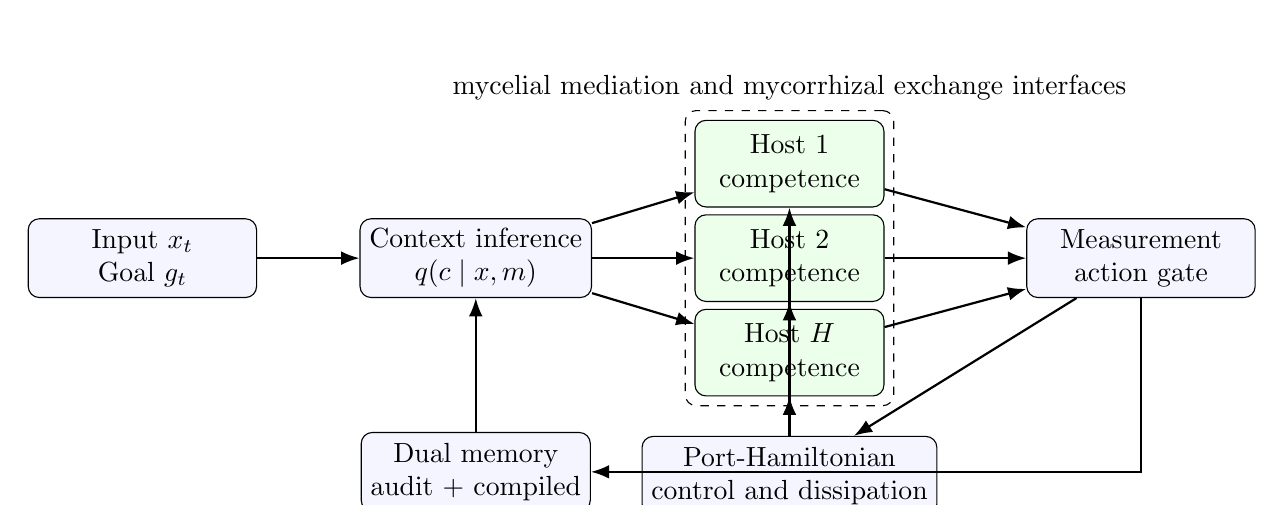
\begin{tikzpicture}[node distance=12mm and 13mm,>=Latex,
box/.style={draw,rounded corners,minimum width=29mm,minimum height=10mm,align=center,fill=blue!4},
host/.style={draw,rounded corners,minimum width=24mm,minimum height=11mm,align=center,fill=green!8},
arrow/.style={->,thick}]
\node[box] (input) {Input $x_t$\\Goal $g_t$};
\node[box,right=of input] (context) {Context inference\\$q(c\mid x,m)$};
\node[host,right=of context,yshift=12mm] (h1) {Host 1\\competence};
\node[host,right=of context] (h2) {Host 2\\competence};
\node[host,right=of context,yshift=-12mm] (h3) {Host $H$\\competence};
\node[box,right=18mm of h2] (measure) {Measurement\\action gate};
\node[box,below=17mm of context] (memory) {Dual memory\\audit + compiled};
\node[box,below=17mm of h2] (control) {Port-Hamiltonian\\control and dissipation};
\draw[arrow] (input)--(context);
\draw[arrow] (context)--(h1);\draw[arrow] (context)--(h2);\draw[arrow] (context)--(h3);
\draw[arrow] (h1)--(measure);\draw[arrow] (h2)--(measure);\draw[arrow] (h3)--(measure);
\draw[arrow] (measure) |- (memory);
\draw[arrow] (memory)--(context);
\draw[arrow] (measure)--(control);
\draw[arrow] (control)--(h1);\draw[arrow] (control)--(h2);\draw[arrow] (control)--(h3);
\node[draw,dashed,rounded corners,fit=(h1)(h2)(h3),label=above:{mycelial mediation and mycorrhizal exchange interfaces}] {};
\end{tikzpicture}
\caption{MMALS architecture. Hosts carry competencies; the mediating network transports signals and resources; interfaces define exchange; memory and control close the loop.}
\label{fig:architecture}
\end{figure}

\section{Theoretical Claims and Boundaries}
\begin{proposition}[Linear-Gaussian boundary]
If an implementation is restricted to Gaussian states, linear symplectic transformations, and Gaussian measurements within the standard efficiently simulable sector, no generic superpolynomial advantage over classical simulation should be expected.
\end{proposition}
\begin{proof}[Justification]
The claim follows by reduction to known Gaussian continuous-variable simulation results \cite{BartlettEtAl2002,WeedbrookEtAl2012}. It is a boundary condition, not a statement about all nonlinear controlled dynamical systems.
\end{proof}

\begin{proposition}[Dissipative convergence under strong convexity]
Assume $u=0$, $J$ is constant, $R\succeq rI$ for $r>0$, and $\mathcal H$ is strongly convex with unique minimizer $Z^\star$. Then $\mathcal H(Z_t)$ is non-increasing and trajectories converge to $Z^\star$ under standard regularity assumptions.
\end{proposition}
\begin{proof}[Sketch]
The energy derivative satisfies $\dot{\mathcal H}\le-r\norm{\nabla\mathcal H}^2$. LaSalle-type arguments and strong convexity identify the invariant set with the unique minimizer.
\end{proof}

\begin{remark}
The convergence proposition is intentionally stronger than realistic neural conditions. It provides a reference theorem against which nonconvex implementations can be evaluated rather than a claim that the full MMALS landscape is convex.
\end{remark}

\section{Experimental Program}
The next empirical phase should test the new model, not retrofit previous results as proof. We propose five experiments.

\subsection{E1: Unitary-to-symplectic equivalence}
Compile small quantum circuits through $\gamma(U)$ and compare complex and real simulations. Metrics: state error, norm preservation, symplectic defect $\norm{S\T JS-J}$, runtime, and precision sensitivity.

\subsection{E2: Transport versus dissipation ablation}
On SplitCIFAR10, RotatedMNIST, and a controlled regime-switching stream, compare: transport only; transport plus fixed damping; learned damping; full port-Hamiltonian control. Metrics: retention, forgetting, route entropy, control energy, settling time, and selector regret.

\subsection{E3: Fisher--Rao versus Euclidean adaptation}
Hold the transport core fixed and compare ordinary gradient, diagonal natural gradient, K-FAC-like approximations, and exact small-scale Fisher updates. Metrics: loss decrease per unit energy, calibration, stability, and context identification.

\subsection{E4: Goal switching and forward--backward control}
Use the existing goal-adaptive branch to switch among accuracy, retention, latency, energy, and risk objectives. Test whether a common dynamics can adapt without changing architectural components.

\subsection{E5: Competence-aware conformal action}
Integrate MMALS-CAL. Compare coverage-only, singleton-only, competence-aware, and risk-aware gates on SplitCIFAR100 and CORe50. The desired outcome is not maximal action rate but a defensible competence--coverage--compactness--context--action tradeoff.

\begin{table}[ht]
\centering
\caption{Minimum evidence bundle for each future run.}
\small
\begin{tabularx}{\textwidth}{p{0.20\textwidth}X}
\toprule
File & Required content\\
\midrule
\texttt{run.json} & immutable run identity, code commit, dataset, seed, hardware, timestamps\\
\texttt{events.jsonl} & stepwise context, route, goal, control, measurement, action, and failure events\\
\texttt{signals.csv} & loss, energy, damping, route entropy, regret, uncertainty, calibration, action\\
\texttt{host\_metrics.csv} & host contribution, dominance, ablation, specialization, stability\\
\texttt{memory.jsonl} & audit and compiled-memory writes, reads, compression, provenance\\
\texttt{summary.json} & aggregate metrics with confidence intervals and validity flags\\
\texttt{figures/} & deterministic reviewer plots generated from the signals\\
\bottomrule
\end{tabularx}
\end{table}

\section{Implementation Pathways}
\subsection{Digital simulation}
The first implementation should use differentiable ordinary differential equations or symplectic integrators \cite{Hairer2006,Greydanus2019}. Structure-preserving integration is essential; otherwise numerical drift can be mistaken for learned dissipation.

\subsection{Continuous-variable photonics}
Photonic quadratures naturally realize symplectic transformations, linear optics, and squeezing. This is a plausible long-term hardware analogy, not evidence of current advantage. Finite squeezing, loss, mode mismatch, non-Gaussian resource cost, and fault-tolerance overhead remain decisive.

\subsection{Classical analog and hybrid control}
Coupled oscillators, electrical networks, and hybrid analog--digital controllers are natural port-Hamiltonian substrates. The realistic near-term contribution is likely resource-efficient control or inference on structured dynamical tasks rather than a general replacement for digital or quantum computers.

\section{Risks of Overinterpretation}
The proposed synthesis has several failure modes:
\begin{enumerate}[leftmargin=*]
\item \textbf{Metaphor inflation:} mycelial language may conceal ordinary mixture-of-experts behavior unless signals and interventions are explicit.
\item \textbf{Geometry without gain:} preserving a symplectic form does not imply improved accuracy, retention, or efficiency.
\item \textbf{Hidden analog resources:} precision and gain may carry the actual computational burden.
\item \textbf{Controller accumulation:} adding $J$, $R$, Fisher updates, calibration, and goals as separate heuristics would reproduce the original fragmentation. They must share a common state and objective account.
\item \textbf{Weak specialization evidence:} routing dominance is not causal specialization.
\item \textbf{Calibration confusion:} valid coverage can coexist with uselessly large prediction sets and almost no safe action.
\item \textbf{Quantum overclaim:} the framework borrows mathematics used in quantum theory but is not thereby quantum, nor does it prove a quantum advantage.
\end{enumerate}

\section{Discussion}
The strongest contribution of the symplectic viewpoint to MMALS is architectural coherence. Reversible transport, dissipative learning, statistical adaptation, control, memory, and measurement become explicit terms of one dynamical system. This directly supports the central MMALS objective: adapt effective complexity to the problem through local rules and energy constraints rather than by stacking ad hoc global controllers.

The framework also clarifies the role of geometry. Fisher--Rao geometry measures change and uncertainty on statistical manifolds. Symplectic geometry organizes directional flow in phase space. They are complementary, not competing. The former answers ``how should beliefs change?''; the latter answers ``how should structured state move?'' Dissipation and control determine what is retained and why.

At the same time, the present article is a foundation paper. It does not report a completed symplectic MMALS benchmark. The evidence table shows why the theory is relevant to existing results, while the experimental section states what must be run before the theory can claim empirical support.

\section{Conclusion}
Volovich's unitary--symplectic observation is mathematically useful but computationally incomplete. By adding explicit dissipation, Fisher--Rao learning, measurement, goal-conditioned control, and finite-resource accounting, it can be transformed into a rigorous foundation for adaptive host networks. For MMALS, the value is not a premature claim that symplectic computers outperform quantum computers. The value is a common mathematical basement in which transport, plasticity, memory, specialization, calibration, and action can be expressed, audited, and experimentally challenged.

\section*{Reproducibility Statement}
The companion repository contains the complete LaTeX source, bibliography, build instructions, Diderot entry payload, magazine chapter, and integration scripts. No new numerical result is claimed in this paper. Program values are labeled as previously reported internal evidence and should be revalidated from immutable evidence bundles before external scientific submission.

\section*{Acknowledgements}
The author acknowledges the MMALS reviewer workflow and the mathematical works cited throughout. Volovich's note is treated as a point of departure, not as an endorsement of its stronger computational claims.

\begin{thebibliography}{99}
\bibitem{Volovich2024} I. V. Volovich, ``Quantum vs. Symplectic Computers,'' \emph{arXiv:2407.12755}, 2024.
\bibitem{Kibble1979} T. W. B. Kibble, ``Geometrization of Quantum Mechanics,'' \emph{Communications in Mathematical Physics}, 65, 189--201, 1979.
\bibitem{AshtekarSchilling1999} A. Ashtekar and T. A. Schilling, ``Geometrical Formulation of Quantum Mechanics,'' in \emph{On Einstein's Path}, Springer, 1999.
\bibitem{RudolphGrover2002} T. Rudolph and L. Grover, ``A 2-Rebit Gate Universal for Quantum Computing,'' \emph{arXiv:quant-ph/0210187}, 2002.
\bibitem{LloydBraunstein1999} S. Lloyd and S. L. Braunstein, ``Quantum Computation over Continuous Variables,'' \emph{Physical Review Letters}, 82, 1784--1787, 1999.
\bibitem{BartlettEtAl2002} S. D. Bartlett, B. C. Sanders, S. L. Braunstein, and K. Nemoto, ``Efficient Classical Simulation of Continuous Variable Quantum Information Processes,'' \emph{Physical Review Letters}, 88, 097904, 2002.
\bibitem{MenicucciEtAl2006} N. C. Menicucci et al., ``Universal Quantum Computation with Continuous-Variable Cluster States,'' \emph{Physical Review Letters}, 97, 110501, 2006.
\bibitem{WeedbrookEtAl2012} C. Weedbrook et al., ``Gaussian Quantum Information,'' \emph{Reviews of Modern Physics}, 84, 621--669, 2012.
\bibitem{GKP2001} D. Gottesman, A. Kitaev, and J. Preskill, ``Encoding a Qubit in an Oscillator,'' \emph{Physical Review A}, 64, 012310, 2001.
\bibitem{VanderSchaft2017} A. van der Schaft and D. Jeltsema, \emph{Port-Hamiltonian Systems Theory: An Introductory Overview}, Now Publishers, 2014.
\bibitem{Rao1945} C. R. Rao, ``Information and the Accuracy Attainable in the Estimation of Statistical Parameters,'' \emph{Bulletin of the Calcutta Mathematical Society}, 37, 81--91, 1945.
\bibitem{Amari1998} S.-i. Amari, ``Natural Gradient Works Efficiently in Learning,'' \emph{Neural Computation}, 10, 251--276, 1998.
\bibitem{AmariNagaoka2000} S.-i. Amari and H. Nagaoka, \emph{Methods of Information Geometry}, AMS, 2000.
\bibitem{Ollivier2015} Y. Ollivier, ``Riemannian Metrics for Neural Networks I: Feedforward Networks,'' \emph{Information and Inference}, 4, 108--153, 2015.
\bibitem{Hairer2006} E. Hairer, C. Lubich, and G. Wanner, \emph{Geometric Numerical Integration}, Springer, 2006.
\bibitem{Greydanus2019} S. Greydanus, M. Dzamba, and J. Yosinski, ``Hamiltonian Neural Networks,'' \emph{NeurIPS}, 2019.
\bibitem{Kirkpatrick2017} J. Kirkpatrick et al., ``Overcoming Catastrophic Forgetting in Neural Networks,'' \emph{PNAS}, 114, 3521--3526, 2017.
\bibitem{Parisi2019} G. I. Parisi et al., ``Continual Lifelong Learning with Neural Networks: A Review,'' \emph{Neural Networks}, 113, 54--71, 2019.
\bibitem{Vovk2005} V. Vovk, A. Gammerman, and G. Shafer, \emph{Algorithmic Learning in a Random World}, Springer, 2005.
\end{thebibliography}
\end{document}
